\documentclass[11pt,a4paper,oneside]{article}
\usepackage{titling}
\newcommand{\subtitle}[1]{%
  \posttitle{%
    \par\end{center}
    \begin{center}\large#1\end{center}
    \vskip0.5em}%
}
\title{\textbf{Group 21: Cognitive Modeling - Lab 3}}
\date{\today}
\author{Olusanmi Hundogan - 6883273\\
Evangelia Giannikou - 6988229\\
}
% \pagenumbering{gobble}
\pagenumbering{arabic}

% \usepackage{eurosym}
\usepackage{hyperref}
% \usepackage{subfig}
\usepackage{amsmath}
\usepackage{amssymb}
\usepackage{tabularx,booktabs}
\usepackage{multicol}
\usepackage{array}
\usepackage{float}
\usepackage[english]{babel}
\usepackage{wrapfig}
\usepackage{graphicx}
\usepackage[font=scriptsize]{caption}
\usepackage{subcaption}


\setcounter{secnumdepth}{0}
\newcolumntype{M}[1]{>{\centering\arraybackslash}m{#1}}
\usepackage[backend=biber, sorting=none]{biblatex}
\usepackage[margin=1in]{geometry}
\addbibresource{references.bib}

\newcommand{\icol}[1]{% inline column vector
  \left(\begin{smallmatrix}#1\end{smallmatrix}\right)%
}

\newcommand{\irow}[1]{% inline row vector
  \begin{smallmatrix}(#1)\end{smallmatrix}%
}

\begin{document}

\maketitle

\section{Question 1}
\label{Q1}
\subsection{$Height \sim \mathcal{N}(180, 10)$}
\textit{Show two graphs: (i) what the probability of using threshold looks like on the scale 1-250 cm; (ii) the graph of the function $\sigma$ on the same scale. State which degree point has the highest probability of being used as a threshold, and on which degree point it is most likely the speaker will use the adjective tall. If the two values differ or are the same, say in a few words why you think this is so.}\\

In Figure \ref{fig:q1_threshold}, the utility of a threshold U on the scale 1-250 cm is shown. The highest degree point is when threshold $ \theta = 0.083$, and height = 184 cm.

\begin{figure}[H]
    \centering
    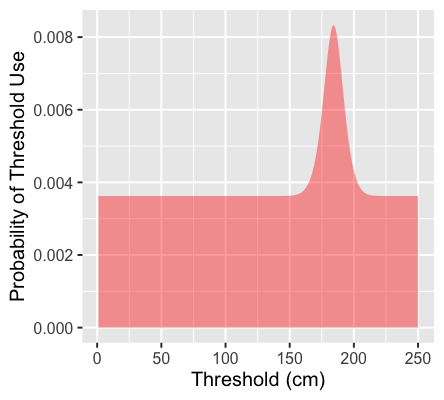
\includegraphics[width=100mm]{figs/Question_1_threshold.png}
    \caption{The graph shows the utility of threshold U on a scale of 1-250 cm.}
  \label{fig:q1_threshold}
\end{figure}

Similarly, in Figure \ref{fig:q1_sigma}, it is shown the graph of the function $\sigma$ on the same scale. The function expresses the likelihood that the speaker will use the adjective 'tall' given a certain degree. In the graph, the highest degree point is 1 and height = 255 cm, which is the optimal. In other words, at this point it is definite that the speaker will use the adjective tall when threshold $ \theta = 1$ and height = 255 cm. As the value decreases, the likelihood is diminishing as well.

\begin{figure}[H]
    \centering
    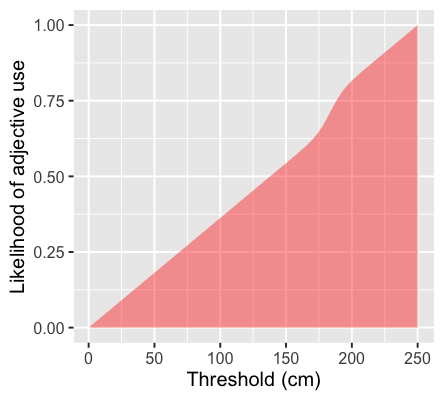
\includegraphics[width=100mm]{figs/Question_1_sigma.png}
    \caption{The graph shows the function $\sigma$ on a scale 1-250 cm.}
  \label{fig:q1_sigma}
\end{figure}

Comparing the two degree points to evaluate the communication efficiency, it is evident that the two values deviate. Considering that $\theta = 1$ is optimal, the speaker is most likely to use the adjective 'tall' for heights greater than 184 cm when $\theta = 0.083$. 

\section{Question 2}
\label{Q2}
\subsection{IQ - normal distribution}
\textit{Specify the normal distribution and generate figures for $ES$ and $\sigma$ function using this distribution and report which degree has the highest $ES$.}\\

$IQ \sim \mathcal{N}(100, 15)$

max value = 0.029 for IQ = 106

\begin{figure}[H]
    \centering
    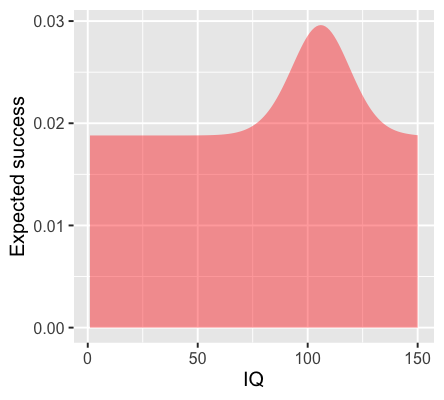
\includegraphics[width=100mm]{figs/Question_2_IQ_es.png}
    \caption{The graph shows the Expected Success function for IQ on a scale of 1-150.}
  \label{fig:q2_iq_es}
\end{figure}

max value = 1 for IQ = 150

\begin{figure}[H]
    \centering
    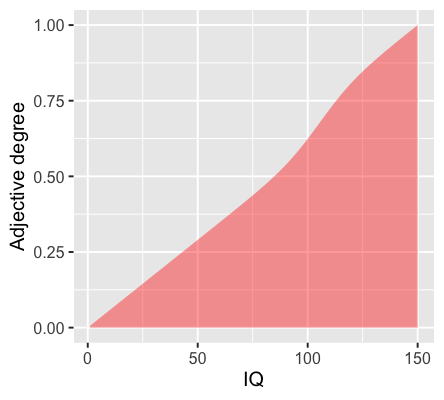
\includegraphics[width=100mm]{figs/Question_2_IQ_sigma.png}
    \caption{The graph shows the $\sigma$ function for IQ on a scale of 1-150.}
  \label{fig:q2_iq_es}
\end{figure}


\subsection{Waiting times - gamma distribution}
\textit{Specify the gamma distribution and generate figures for $ES$ and $\sigma$. Report which degree has the highest $ES$.}\\

Waiting times $\sim \mathcal{\gamma}(2, 1)$
$max value = 0.3874$ for $waiting time = 2$

\begin{figure}[H]
    \centering
    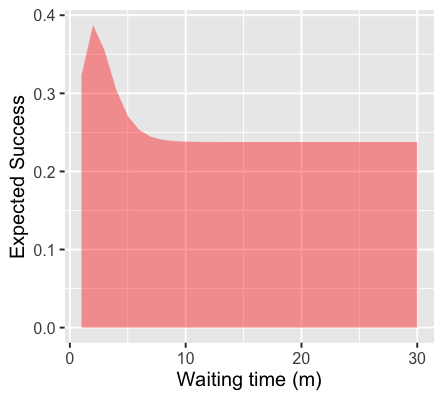
\includegraphics[width=100mm]{figs/Question_2_waiting_time_es.png}
    \caption{The graph shows the $\sigma$ function for waiting on a scale of 1-30.}
  \label{fig:q2_iq_sigma}
\end{figure}

$max value = 1$ for $waiting time = 30$
\begin{figure}[H]
    \centering
    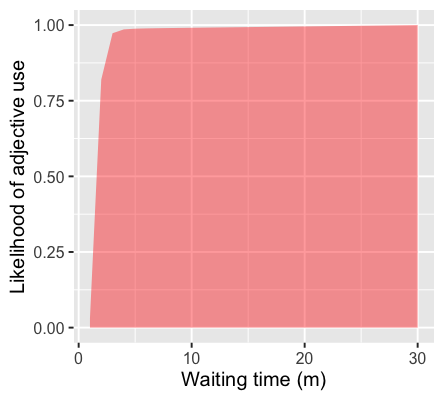
\includegraphics[width=100mm]{figs/Question_2_waiting_time_sigma.png}
    \caption{The graph shows the $\sigma$ function for waiting on a scale of 1-30.}
  \label{fig:q2_iq_sigma}
\end{figure}

\section{Question 3}
\label{Q3}
\textit{What is Pearson’s correlation coefficient, r, between model’s predictions and actual observations. Check the value of $r$ with respect to three different parameters of the model (9 comparisons in total):}

\begin{itemize}
    \item \textit{lambda=40, coverage.parameter=0.1}
    \item \textit{lambda=40, coverage.parameter=-0.1}
    \item \textit{lambda=40, coverage.parameter=0}
\end{itemize}

\textit{What coverage parameter gives us the best and the worst linear correlation? On which distribution do we get the best results?}

\textit{Afterward, pick the coverage parameter that worked best and select two distributions by flipping their prior belief distributions. Report what prior distribution you used and report r. Do we see that r is affected? Does the model suffer in having worse linear correlation with respect to the observed data? Say in a few words why this is the case.}\\

As it is visible in Table \ref{question_3}, the best linear correlation is given when the coverage parameter is -0.1 where on average $r = 0.85$. The worst correlation is given when coverage parameter is 0.1 where on average $r = 0.74$.

Similarly, when comparing the results between the distribution, the best correlation is that of the Gaussian with an average $r = 0.93$. The worst correlation is given for the Left-skewed distribution where on average $r = 0.55$.

\begin{table}[ht]
\centering
\begin{tabular}{rccc}
  \hline
 Model & $c = 0.1$ & $c = -0.1$ & $c = 0$ \\ 
  \hline
    Gaussian & 0.88 & 0.97 & 0.94\\ 
    Left - skewed & 0.85 & 0.98 & 0.98\\ 
    Moved & 0.84 & 0.97 & 0.93\\ 
   \hline
\end{tabular}
\caption{Pearson's correlation between model's prediction and actual observation for 3 different model distributions where $\lambda = 40$ and coverage parameter is 0.1, -0.1 and 0.}
\label{question_3}
\end{table}

For the second part of the question, we picked $c = -0.1$ as the best coverage parameter and selected to flip the distribution of the left-skewed and moved models. In particular, we used normal distribution with $mean = 6$ and $st.d = 2$ for the left-skewed model. The correlation we found was $r = 0.93$. For the moved model we used gamma distribution with $shape = 4$ and $scale = 1.5$. The correlation found was $r = 0.35$.

A sum of the results in regards to the previously observed data is found on Table \ref{question_3_flipped}. In the case of the left-skewed model, the correlation improves a lot with a prior distribution set. In contrast, for the moved model, the correlation worsens. This decrease was expected since gamma distribution would not work well with data that are concentrated on the right side of distribution.
% [TO-DO: explain why this happens even more?!]

\begin{table}[ht]
\centering
\begin{tabular}{rccr}
  \hline
 Model & r with Normal distribution & r with Gamma distribution\\ 
  \hline
    Left - skewed & 0.95* & 0.98 \\ 
    Moved & 0.97 & 0.86* \\ 
   \hline
\end{tabular}
\caption{Pearson's correlation between 2 models with $c = -0.1$. The * indicates the new correlation values with flipped distribution.}
\label{question_3_flipped}
\end{table}

\section{Question 4}
\label{Q4}
\textit{Bayesian model - What values have been found for lambda and coverage.parameter? Report summary statistics on lambda and coverage.parameter (MAP, median, 2.5\% to 97.5\%). Discuss briefly the summaries.}\\

As seen in Table \ref{question_4},  the values of 2.5\% and 97.5\% interval indicate the limits of c and $\lambda$. In other words, there is a 95\% chance that the coverage parameter value will be between 0.380 - 0.981 and lambda between 17.242 - 44.654. This is in agreement with the MAP value which is 0.793 for c and 21.400 for $\lambda$.

\begin{table}[ht]
\centering
\begin{tabular}{ccccc}
  \hline
  & MAP & 2.5\% interval & median & 97.5\% interval\\ 
  \hline
    c & 0.793 & 0.380 & 0.600 & 0.981\\ 
    $\lambda$ & 21.400 & 17.242 & 28.134 & 44.654\\ 
   \hline
\end{tabular}
\caption{A statistics summary of c and $\lambda$ for adjective='big' on a Gaussian distribution.}
\label{question_4}
\end{table}

%[TO-DO: discuss - are values in out widespread or very narrow? If so, why do you think this is the case and is it good/bad?]

\section{Question 5}
\label{Q5}
\textit{Expand your model to construct the posterior distribution of the two parameters using three adjectives (big, pointy, tall) in all three distributions. Explore the distribution of the parameters in out. Plot the summary and report summary statistics on lambda and coverage.parameter.}\\

\begin{table}[ht]
\centering
\begin{tabular}{ccccc}
  \hline
  & MAP & 2.5\% interval & median & 97.5\% interval\\ 
  \hline
    c & 0.853 & 0.392 & 0.569 & 0.925\\ 
    $\lambda$ & 19.947 & 18.410 & 29.767 & 43.406\\ 
   \hline
\end{tabular}
\caption{A statistics summary of c and $\lambda$ for adjectives = 'big', 'pointy', 'tall' for 3 distributions.}
\label{question_4}
\end{table}

\section{Bonus question}
\label{bonus}
\textit{We specified the likelihood using dnorm with $sd=0.1$. Is this sensible or not? Check what dnorm is and state what problems there might be with this particular function and with $sd=0.1$ for our data. Is there an alternative probability distribution that would make more sense?}\\

\clearpage 
\printbibliography
\end{document}